\chapter{RET}
	\section{Prezentacja urządzenia}
		Na poniższym rysunku przedstawiono RET-a czyli urządzenie dla którego zaimplementowano symulator sterownika.\cite{KATHREIN_RET_1}
		\begin{figure}[h!]
		\centering
		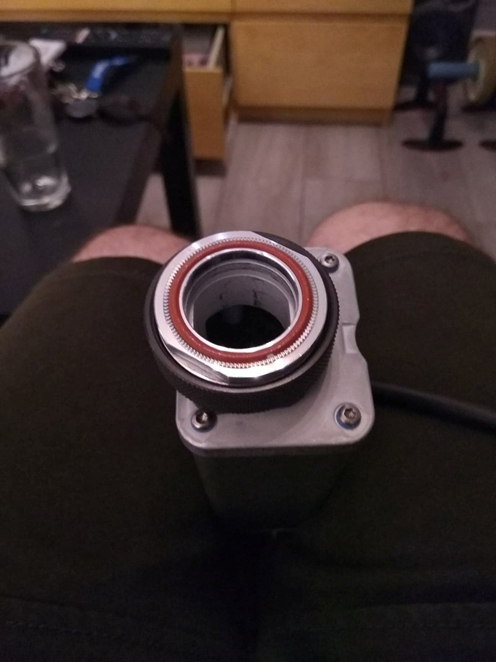
\includegraphics[scale=0.4]{Obrazki/RET_1.png}
		\caption{RET - Miejsce na antenę, zdjęcie własne}
		\end{figure}

		\begin{figure}[h!]
		\centering
		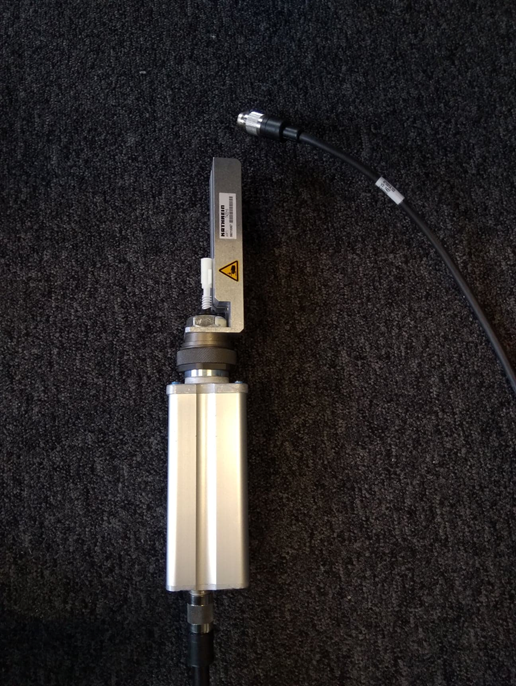
\includegraphics[scale=0.4]{Obrazki/RET_2.png}
		\caption{RET - podłączonym kablem RS-485 oraz włożoną atrapą anteny, zdjęcie własne}
		\end{figure}

	\section{Zmiana szerokości głównej wiązki fali elektromagnetycznej}
		\begin{figure}[h!]
		\centering
		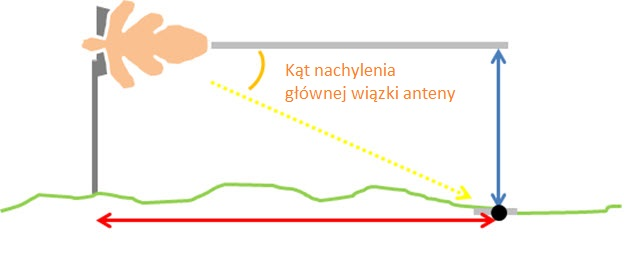
\includegraphics[scale=1.0]{Obrazki/Angle.jpeg}
		\caption{Rysunek przedstawiający kąt modyfikowany przy pomocy RET-a}
		\end{figure}
		
		Poniższe rysunki wygenerowano dzięki programowi Radio Mobile\cite{RADIO_MOBILE_PAGE_1},
		Przedstawiono na nich szerokość wiązki promieni sygnału radiowego w osi poziomej\cite{BEAMWIDTH_1}
		zmieniającą się dzięki modyfikacji elektrycznego kąta na wartość 40-tu stopni.
		Podczas symulacji użyto antenę Yagi, która aktualnie nie jest stosowana w technologii mobilnej z racji wspieranych
		przez nią częstotliwości, gdyż są one znacznie niższe aniżeli te wymagane przez WCDMA, LTE czy \textit{5G}, 
		aczkolwiek bardzo dobrze odzwierciedla działanie tych rzeczywistych ze względu na swoją charakterystykę kierunkową.
		\newline
		Antenę umieszczono przy WSIZ Copernicus. \newline
		Pomarańczowym kolorem przedstawiono charakterystykę zysku promieniowania anteny, które w przypadku kąta 0 stopni jest wydłużone oraz węższe,
		co pozwala pokryć śladowym zasięgiem nawet dalekie obszary, lecz do terenów bliżej zlokolizowanych dostarczony
		jest słabszy sygnał względem tego, który można otrzymać, zmieniając elektryczny kąt anteny na 40 stopni.
		Dzięki RET-owi, można skoncentrować wiązkę na mniejszym obszarze, oferując znacznie wyższe prędkości transmisji danych.

		\begin{figure}[h!]
		\centering
		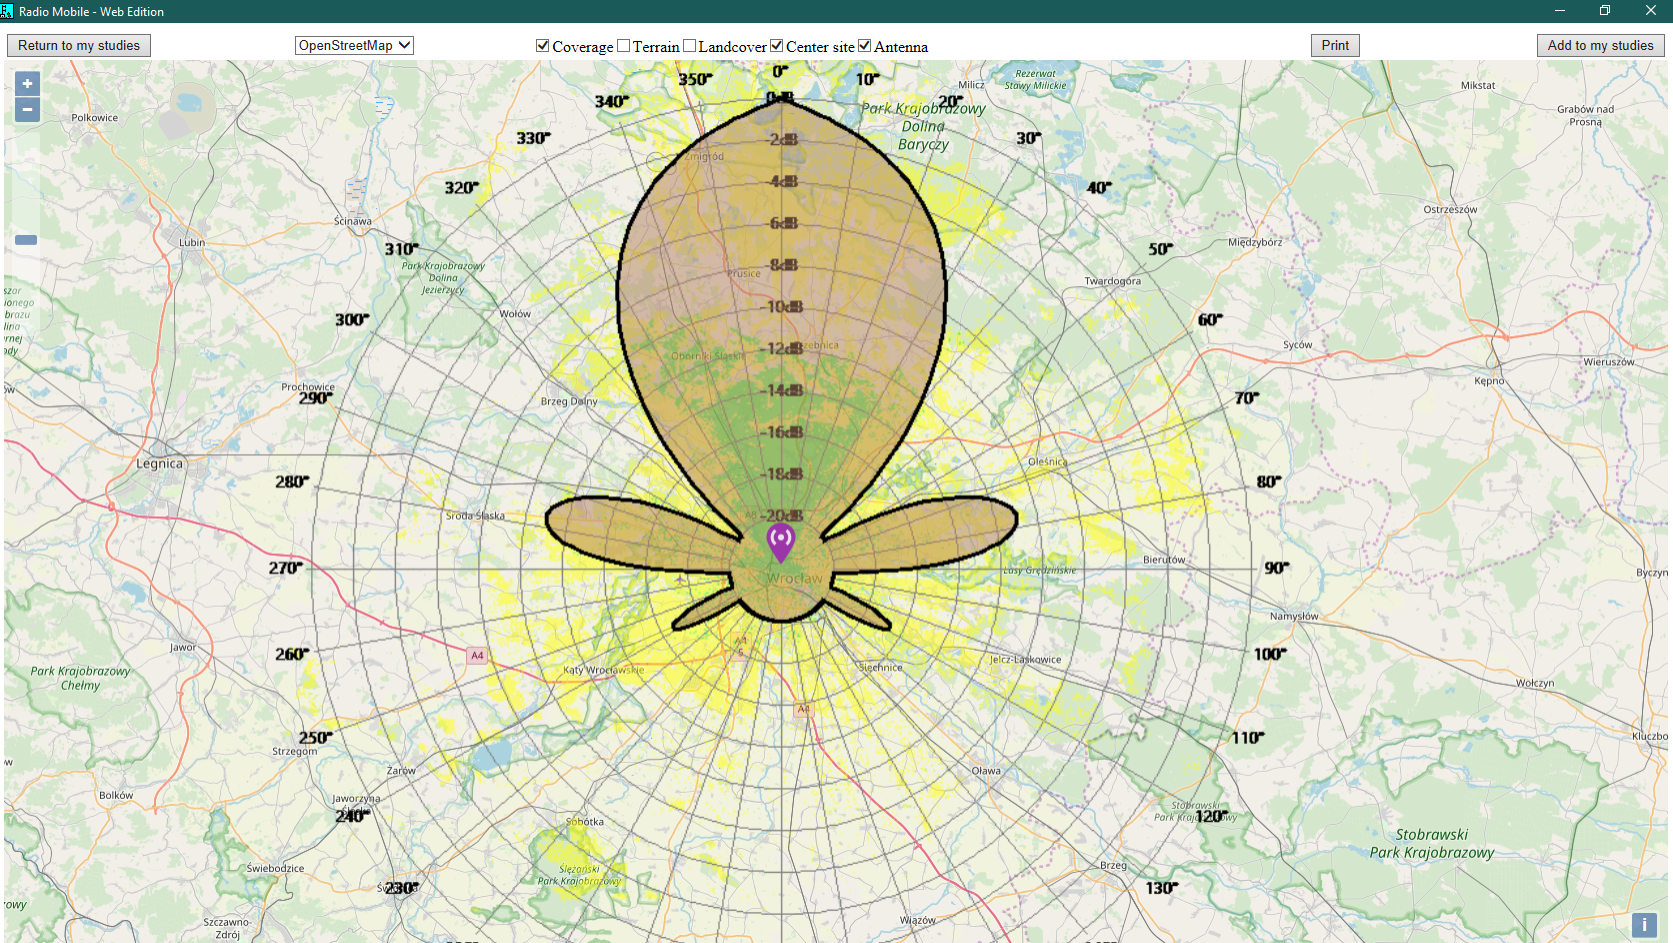
\includegraphics[scale=0.5]{Obrazki/Antenna_Yagi_Angle_0.png}
		\caption{Pokrycie obszaru sygnałem radiowym dzięki antenie Yagi, kąt elektryczny 0 stopni}
		\end{figure}

		\begin{figure}[h!]
		\centering
		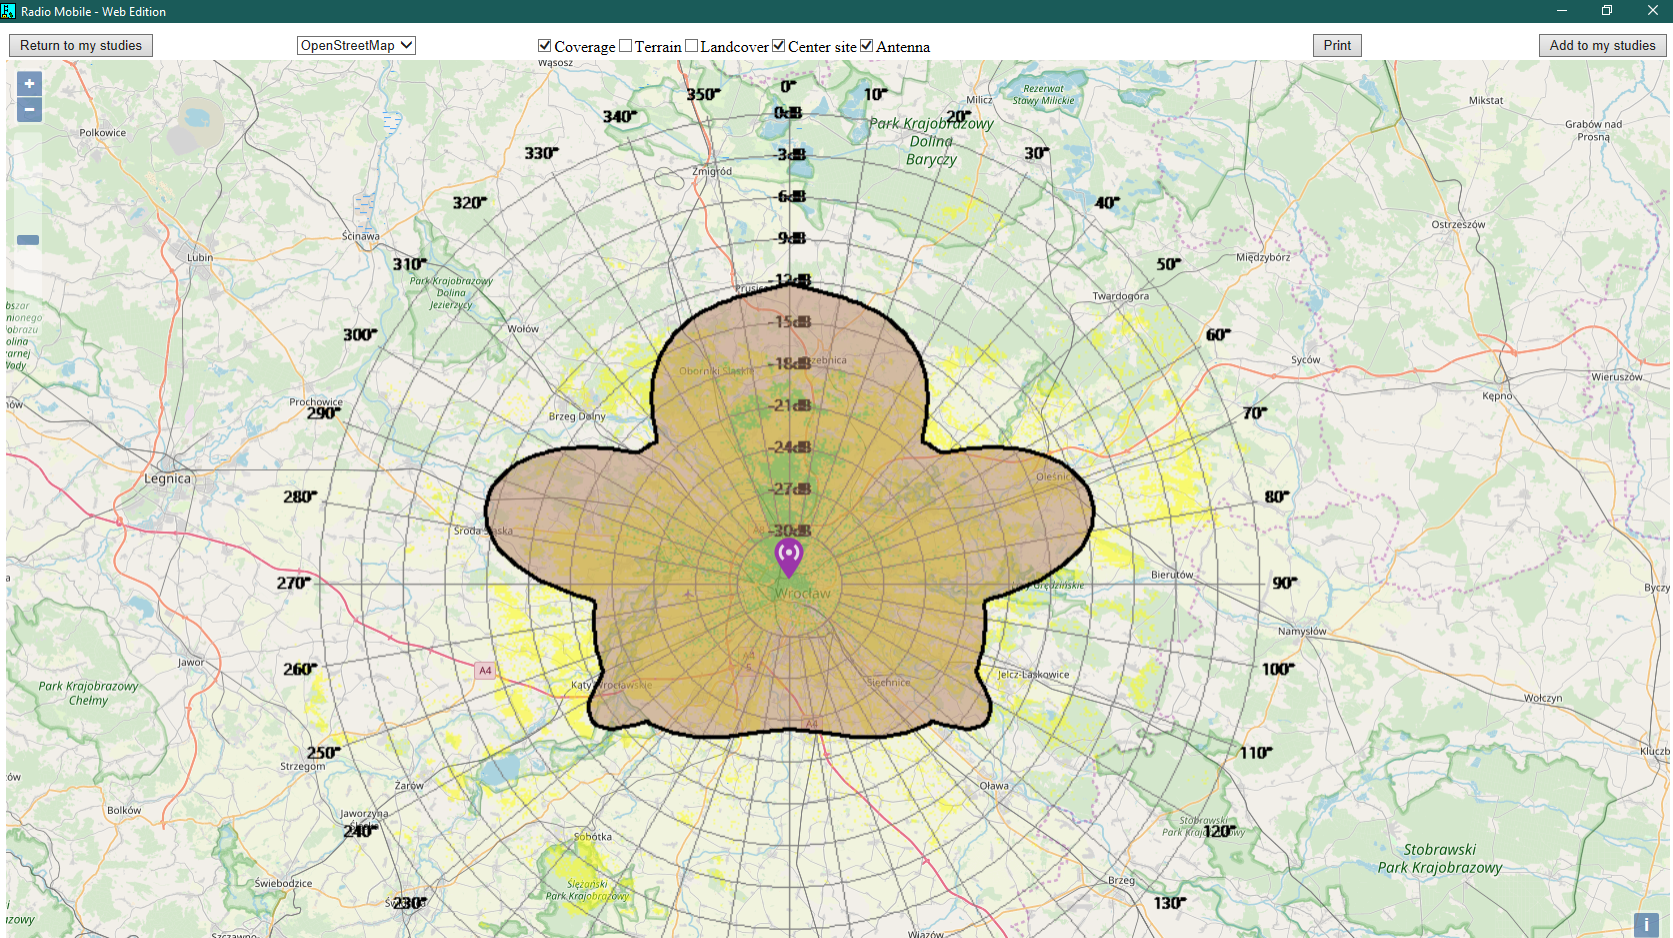
\includegraphics[scale=0.5]{Obrazki/Antenna_Yagi_Angle_40.png}
		\caption{Pokrycie obszaru sygnałem radiowym dzięki antenie Yagi, kąt elektryczny 40 stopni}
		\end{figure}
